\appendix

\subsection{Qualitative Results}
\begin{figure*}[!t]
  \centering
   \includegraphics[width=.94 \linewidth]{figure/cfg_conparision.png}
    \caption{Results using no CFG, standard CFG, and R-CFG with Self-Negative and Onetime-Negative approaches. When compared to cases where CFG is not utilized, the cases with CFG utilized can intensify the impact of prompts. In the proposed method R-CFG, a more pronounced influence of prompts was observed. Both CFG and R-CFG use guidance scale $\gamma = 1.4$. For R-CFG, the first two rows use magnitude modelation coefficient $\delta = 1.0$, and the third row uses $\delta=0.5$.}
\label{fig:cfg_conparision}
\end{figure*}

\begin{figure*}[!t]
  \centering
   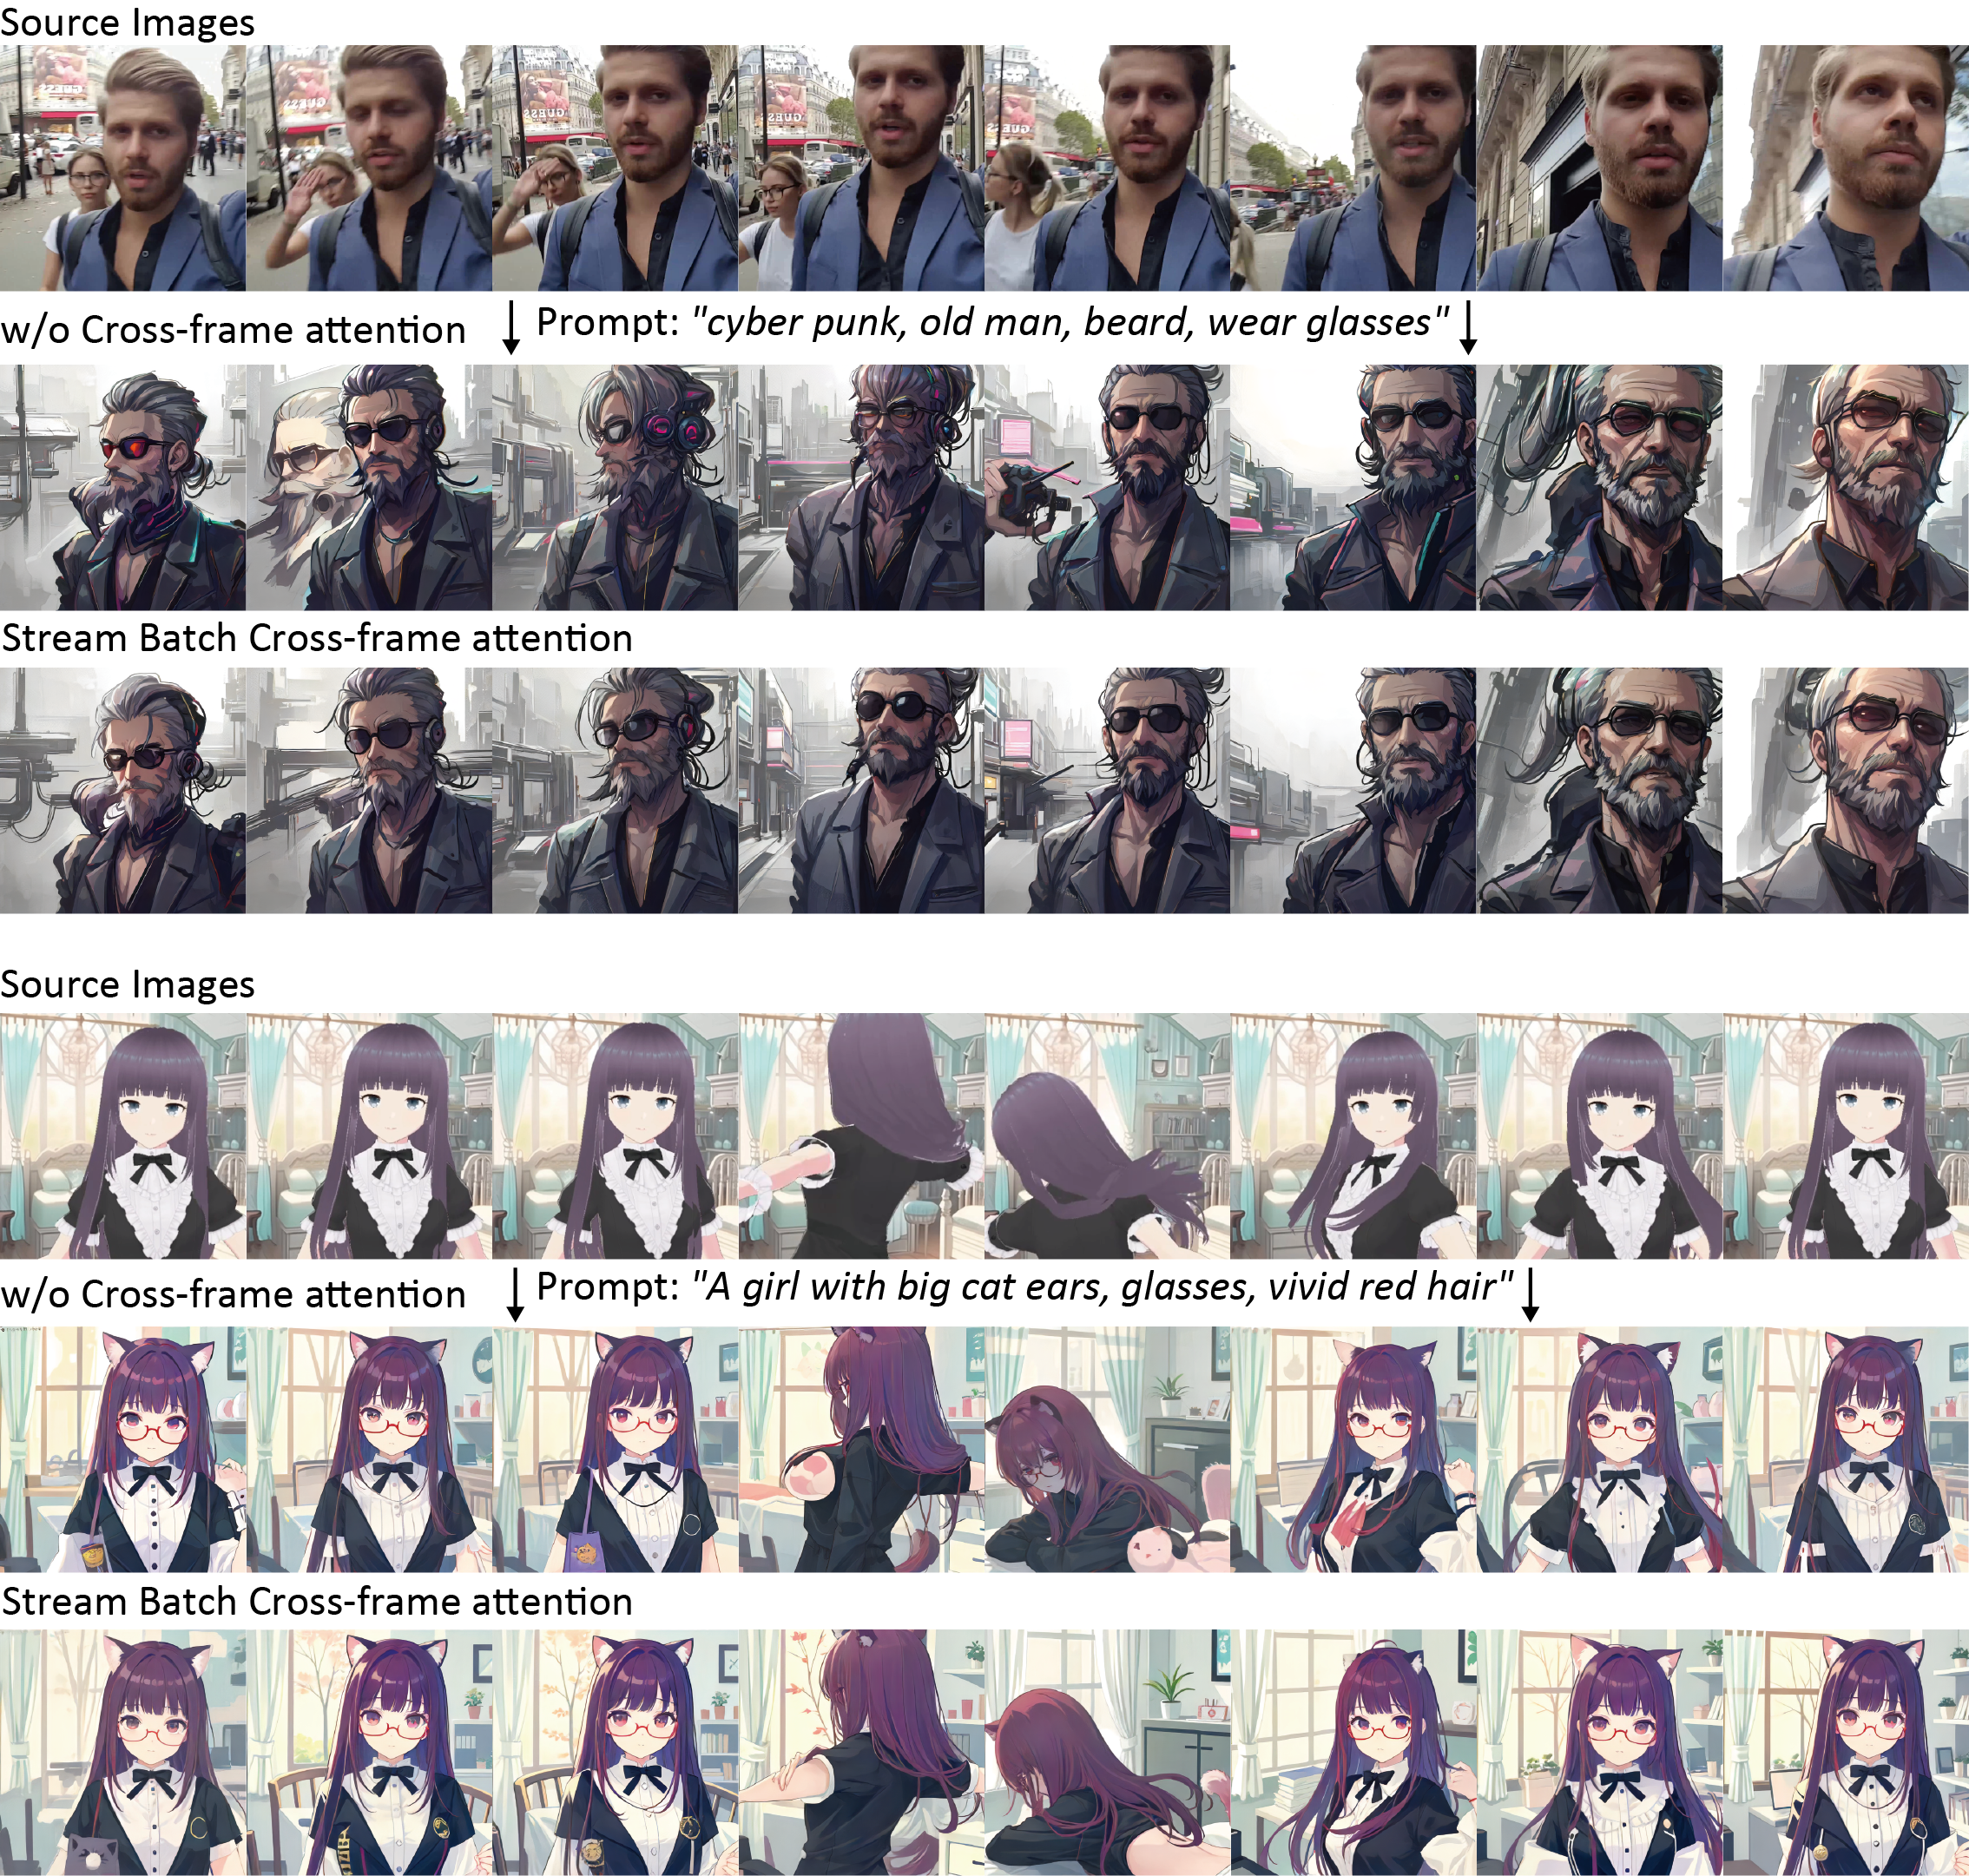
\includegraphics[width=\linewidth]{figure/time_consistency_evaluation.png}
\caption{Time consistency qualitative evaluation: In cases where the subject's face moves significantly in intermediate frames, it can be observed that using StreamBatch Cross-frame attention produces more appropriate and temporally consistent generation results by leveraging the context from preceding and succeeding frames.}
\label{fig:time_vis}
\end{figure*}


\section{More Architecture details}

\subsection{Input-Output Queue}

\begin{figure*}[!t]
  \centering
   \includegraphics[width=.9\linewidth]{figure/queue_concept.png}
\caption{Input-Output Queue: The process of converting input images into a tensor data format manageable by the pipeline, and conversely, converting decoded tensors back into output images requires a non-negligible amount of additional processing time. To avoid adding these image processing times to the bottleneck process, the neural network inference process, we have segregated image pre-processing and post-processing into separate threads, allowing for parallel processing. Moreover, by utilizing an Input Tensor Queue, we can accommodate temporary lapses in input images due to device malfunctions or communication errors, enabling smooth streaming.}
\label{fig:queue_para}
\end{figure*}

The current bottleneck in high-speed image generation systems lies in the neural network modules, including VAE and U-Net. To maximize the overall system speed, processes such as pre-processing and post-processing of images, which do not require handling by the neural network modules, are moved outside of the pipeline and processed in parallel.

In the context of input image handling, specific operations, including resizing of input images, conversion to tensor format, and normalization, are meticulously executed. To address the disparity in processing frequencies between the human inputs and the model throughput, we design an input-output queuing system to enable efficient parallelization, as shown in Fig. \ref{fig:queue_para}. This system operates as follows: processed input tensors are methodically queued for Diffusion Models. During each frame, Diffusion Model retrieves the most recent tensor from the input queue and forwards it to the VAE Encoder, thereby triggering the image generation sequence. Correspondingly, tensor outputs from the VAE Decoder are fed into an output queue. In the subsequent output image handling phase, these tensors are subject to a series of post-processing steps and conversion into the appropriate output format. Finally, the fully processed image data is transmitted from the output handling system to the rendering client.



\subsection{Pre-computation}
The U-Net architecture requires both input latent variables and conditioning embeddings. Typically, the conditioning embedding is derived from a text prompt, which remains constant across different frames. To optimize this, we pre-compute the prompt embedding and store it in a cache. In interactive or streaming mode, this pre-computed prompt embedding cache is recalled. 
Within U-Net, the Key and Value are computed based on this pre-computed prompt embedding for each frame. We have modified the U-Net to store these Key and Value pairs, allowing them to be reused. Whenever the input prompt is updated, we recompute and update these Key and Value pairs inside U-Net.

For consistent input frames across different timesteps and to improve computational efficiency, we pre-sample Gaussian noise for each denoising step and store it in the cache. This approach is particularly relevant for image-to-image tasks.

We also precompute \(\alpha_{\tau}\) and \(\beta_{\tau}\), the noise strength coefficients for each denoising step \(\tau\), defined as:

\begin{equation}
x_t = \sqrt{\alpha_{\tau}}x_0 + \sqrt{\beta_{\tau}}\epsilon
\end{equation}
\label{eq:fw_diffusion_process}

This is a minor point in low throughput scenarios, but at frame rates higher than 60 FPS, the overhead of recomputing these static values becomes noticeable.

We note that we have a specific design for the inference parameterization for latent consistency models (LCM). As per the original paper, we need to compute \(c_\mathrm{skip}(\tau)\) and \(c_\mathrm{out}(\tau)\) to satisfy the following equation:

\begin{equation}
f_\theta(x,\tau) = c_\mathrm{skip}(\tau)x + c_\mathrm{out}(\tau)F_\theta(x,\tau).
\end{equation}
\label{eq:cm_parameterization}

The functions \(c_\mathrm{skip}(\tau)\) and \(c_\mathrm{out}(\tau)\) in original LCM \cite{luo2023lcm} is constructed as follows:

\begin{equation}
c_\mathrm{skip}(\tau)=\frac{\sigma_\mathrm{data}^2}{(s\tau)^2+\sigma_\mathrm{data}^2}, \quad c_\mathrm{out}(\tau)=\frac{\sigma_\mathrm{data}s\tau}{\sqrt{\sigma_\mathrm{data}^2+(s\tau)^2}},
\end{equation}
\label{eq:c_skip_c_out}

where \(\sigma_{\mathrm{data}}=0.5\), and the timestep scaling factor \(s=10\). We note that with \(s=10\), \(c_\mathrm{skip}(\tau)\) and \(c_\mathrm{out}(\tau)\) approximate delta functions that enforce the boundary condition to the consistency models. (i.e., at denoising step \(\tau=0\), \(c_\mathrm{skip}(0)=1\), \(c_\mathrm{out}(0)=0\); and at \(\tau\neq0\), \(c_\mathrm{skip}(\tau)=0\), \(c_\mathrm{out}(\tau)=1\)). At inference time, there's no need to recompute these functions repeatedly. We can either pre-compute \(c_\mathrm{skip}(\tau)\) and \(c_\mathrm{out}(\tau)\) for all denoising steps \(\tau\) in advance or simply use constant values \(c_\mathrm{skip}=0\), \(c_\mathrm{out}=1\) for any arbitrary denoising step \(\tau\).


\subsection{Model Acceleration and Tiny AutoEncoder}
% \cfx{I suggest putting this to Experiment part}
We employ TensorRT to construct the U-Net and VAE engines, further accelerating the inference speed. TensorRT is an optimization toolkit from NVIDIA that facilitates high-performance deep learning inference. It achieves this by performing several optimizations on neural networks, including layer fusion, precision calibration, kernel auto-tuning, dynamic tensor memory, and more. These optimizations are designed to increase throughput and efficiency for deep learning applications.

To optimize speed, we configured the system to use static batch sizes and fixed input dimensions (height and width). This approach ensures that the computational graph and memory allocation are optimized for a specific input size, leading to faster processing times. However, this means that if there is a requirement to process images with different shapes (i.e., varying heights and widths) or to use different batch sizes (including those for denoising steps), a new engine tailored to these specific dimensions must be built. This is because the optimizations and configurations applied in TensorRT are specific to the initially defined dimensions and batch size, and changing these parameters would necessitate a reconfiguration and re-optimization of the network within TensorRT.

Besides, we employ a tiny AutoEncoder, which has been engineered as a streamlined and efficient counterpart to the traditional Stable Diffusion AutoEncoder \cite{kingma2022autoencoding, rombach2021highresolution}. TAESD excels in rapidly converting latents into full-size images and accomplishing decoding processes with significantly reduced computational demands. 


\section{Text-to-Image Quality}
The quality of standard text-to-image generation results is demonstrated in Fig. \ref{fig:txt2img_results}. Using the sd-turbo model, high-quality images like those shown in Fig. \ref{fig:txt2img_results} can be generated in just one step. When images are produced using our proposed StreamDiffusion pipeline and SD-turbo model in an environment with GPU: RTX 4090, CPU: Core i9-13900K, and OS: Ubuntu 22.04.3 LTS, it's feasible to generate such high-quality images at a rate exceeding 100fps. Furthermore, by increasing the batch size of images generated at once to 12, our pipeline can continuously produce approximately 150 images per second.
The images enclosed in red frames shown in Fig. \ref{fig:txt2img_results} are generated in four steps using community models merged with LCM-LoRA. While these LCM models require more than 1 step for high quality image generation, resulting in a reduction of speed to around 40fps, these LCM-LoRA based models offer the flexibility of utilizing any base model, enabling the generation of images with diverse expressions.

\begin{figure*}[!t]
  \centering
   \includegraphics[width=.9\linewidth]{figure/txt2img_result.png}
\caption{Text-to-Image generation results. We use four step denoising for LCM-LoRA, and one step denoising for sd-turbo. Our StreamDiffusion enables the real-time generation of images with quality comparable to those produced using Diffusers AutoPipeline Text2Image.}
\label{fig:txt2img_results}
\end{figure*}


\section{GPU Usage Under Dynamic Scene}

We also evaluate the GPU usage under dynamic scenes on one RTX 4090 GPU, as shown in the Figure. \ref{fig:gpu_usage_4090}. The analysis of the GPU usage is shown in Section 4.2 of the main text. 
\begin{figure*}[!t]
    \centering
    \includegraphics[width=.9\linewidth]{figure/gpu_utilization-paper.png}
    \vspace{-5mm}
    \caption{GPU Usage comparison under static scene. (GPU: RTX3060, Number of frames: 20) The blue line represents the GPU usage with SSF, the orange line indicates GPU usage without SSF, and the red line denotes the Skip probability calculated based on the cosine similarity between input frames. Additionally, the top of the plot displays input images corresponding to the same timestamps. In this case, the character in the input images is only blinking.}
    \label{fig:gpu_usage_3090}
    \vspace{-10mm}
\end{figure*}

\begin{figure*}[!t]
  \centering
   \includegraphics[width=.9\linewidth]{figure/gpu_utilization_RTX4090_1000frames.png}
\caption{GPU Usage comparison under dynamic scene. (GPU: RTX4090, Number of frames: 1000) The blue line represents the GPU usage with SSF, the orange line indicates GPU usage without SSF, and the red line denotes the Skip probability calculated based on the cosine similarity between input frames. Additionally, the top of the plot displays input images corresponding to the same timestamps. In this case, the character in the input images keeps moving dynamically. Thus, this analysis compares GPU usage in a dynamic scenario.}
\label{fig:gpu_usage_4090}
\end{figure*}